\documentclass{standalone}
\usepackage{tikz}
\usetikzlibrary{patterns, positioning}


\begin{document}
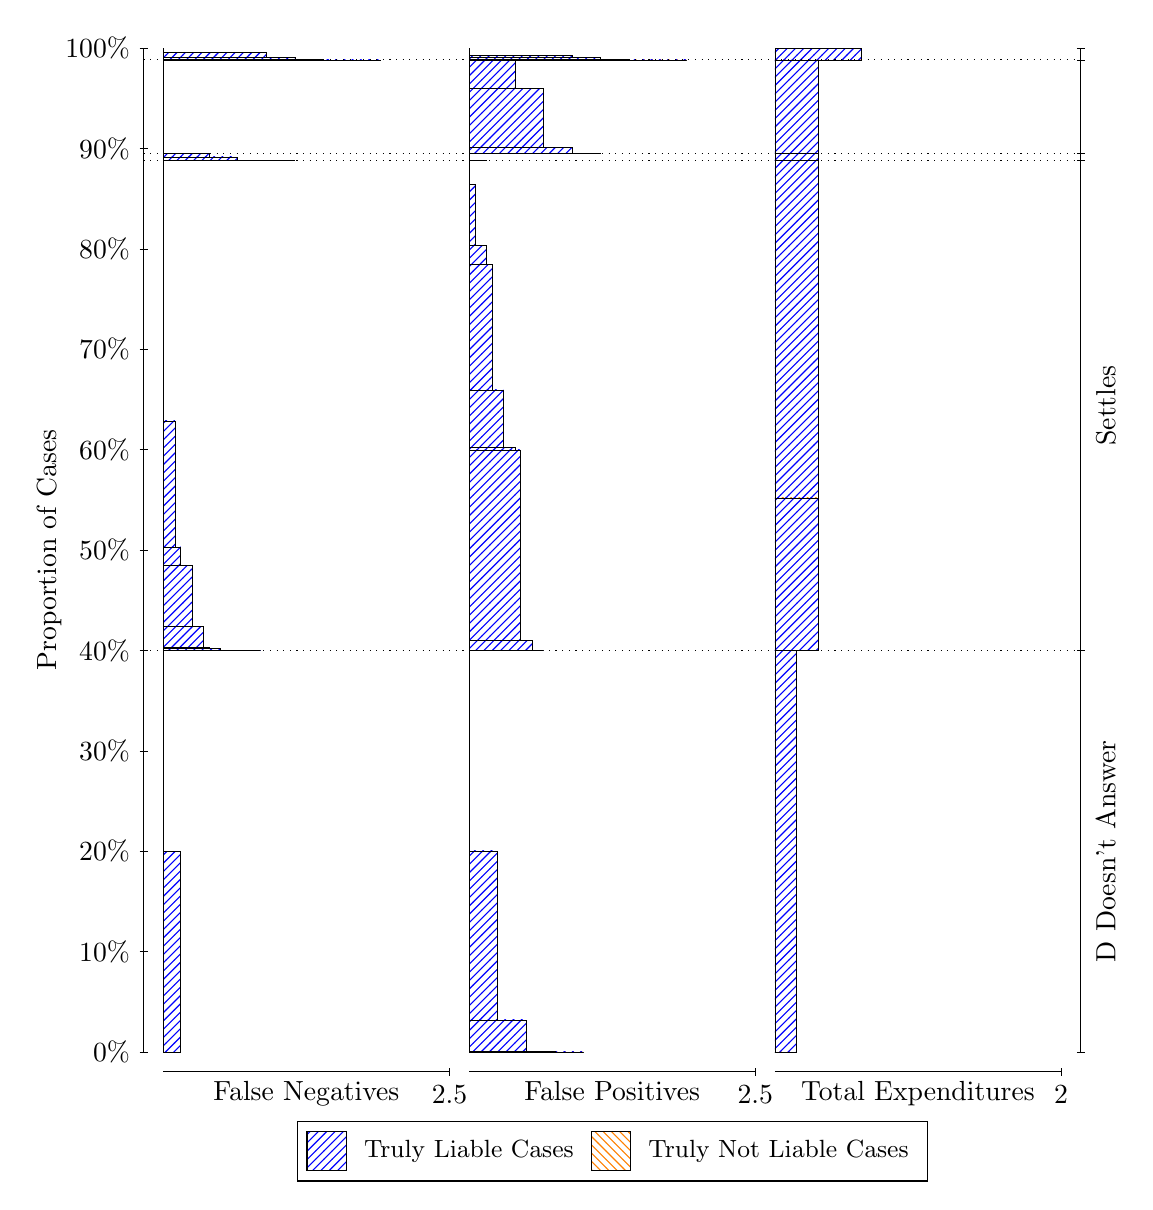
\begin{tikzpicture}
\draw[black, very thin] (1.5,1.75) -- (1.5,14.5);
\node[rotate=90, text=black, anchor=center] at (0.3, 8.125) {Proportion of Cases};
\draw[black, very thin] (1.45,1.75) -- (1.55,1.75);
\node[text=black, anchor=east] at (1.45, 1.75) {0\%};
\draw[black, very thin] (1.45,3.025) -- (1.55,3.025);
\node[text=black, anchor=east] at (1.45, 3.025) {10\%};
\draw[black, very thin] (1.45,4.3) -- (1.55,4.3);
\node[text=black, anchor=east] at (1.45, 4.3) {20\%};
\draw[black, very thin] (1.45,5.575) -- (1.55,5.575);
\node[text=black, anchor=east] at (1.45, 5.575) {30\%};
\draw[black, very thin] (1.45,6.85) -- (1.55,6.85);
\node[text=black, anchor=east] at (1.45, 6.85) {40\%};
\draw[black, very thin] (1.45,8.125) -- (1.55,8.125);
\node[text=black, anchor=east] at (1.45, 8.125) {50\%};
\draw[black, very thin] (1.45,9.4) -- (1.55,9.4);
\node[text=black, anchor=east] at (1.45, 9.4) {60\%};
\draw[black, very thin] (1.45,10.675) -- (1.55,10.675);
\node[text=black, anchor=east] at (1.45, 10.675) {70\%};
\draw[black, very thin] (1.45,11.95) -- (1.55,11.95);
\node[text=black, anchor=east] at (1.45, 11.95) {80\%};
\draw[black, very thin] (1.45,13.225) -- (1.55,13.225);
\node[text=black, anchor=east] at (1.45, 13.225) {90\%};
\draw[black, very thin] (1.45,14.5) -- (1.55,14.5);
\node[text=black, anchor=east] at (1.45, 14.5) {100\%};

\draw[black, very thin] (13.4,1.75) -- (13.4,14.5);
\draw[black, very thin] (13.35,1.75) -- (13.45,1.75);
\node[anchor=west] at (13.35, 1.75) {};
\draw[black, very thin] (13.35,6.8488) -- (13.45,6.8488);
\node[anchor=west] at (13.35, 6.8488) {};
\draw[black, very thin] (13.35,13.073) -- (13.45,13.073);
\node[anchor=west] at (13.35, 13.073) {};
\draw[black, very thin] (13.35,13.159) -- (13.45,13.159);
\node[anchor=west] at (13.35, 13.159) {};
\draw[black, very thin] (13.35,14.349) -- (13.45,14.349);
\node[anchor=west] at (13.35, 14.349) {};
\draw[black, very thin] (13.35,14.5) -- (13.45,14.5);
\node[anchor=west] at (13.35, 14.5) {};

\draw[black, very thin, pattern color=blue, pattern=north east lines] (1.75,1.75) rectangle (1.968,4.2958);
\draw[black, very thin, pattern color=orange, pattern=north west lines] (1.75,4.2958) rectangle (1.75,4.2958);
\draw[black, very thin, pattern color=blue, pattern=north east lines] (1.75,4.2958) rectangle (1.75,6.8488);
\draw[black, very thin, pattern color=blue, pattern=north east lines] (1.75,6.8488) rectangle (2.9853,6.8488);
\draw[black, very thin, pattern color=blue, pattern=north east lines] (1.75,6.8488) rectangle (2.84,6.8488);
\draw[black, very thin, pattern color=blue, pattern=north east lines] (1.75,6.8488) rectangle (2.6947,6.8488);
\draw[black, very thin, pattern color=blue, pattern=north east lines] (1.75,6.8488) rectangle (2.622,6.8533);
\draw[black, very thin, pattern color=blue, pattern=north east lines] (1.75,6.8533) rectangle (2.4767,6.8797);
\draw[black, very thin, pattern color=blue, pattern=north east lines] (1.75,6.8797) rectangle (2.3313,6.8915);
\draw[black, very thin, pattern color=blue, pattern=north east lines] (1.75,6.8915) rectangle (2.2587,7.1547);
\draw[black, very thin, pattern color=blue, pattern=north east lines] (1.75,7.1547) rectangle (2.1133,7.9288);
\draw[black, very thin, pattern color=blue, pattern=north east lines] (1.75,7.9288) rectangle (1.968,8.1651);
\draw[black, very thin, pattern color=blue, pattern=north east lines] (1.75,8.1651) rectangle (1.8953,9.7635);
\draw[black, very thin, pattern color=orange, pattern=north west lines] (1.75,9.7635) rectangle (1.75,9.7635);
\draw[black, very thin, pattern color=blue, pattern=north east lines] (1.75,9.7635) rectangle (1.75,13.073);
\draw[black, very thin, pattern color=blue, pattern=north east lines] (1.75,13.073) rectangle (3.4213,13.073);
\draw[black, very thin, pattern color=blue, pattern=north east lines] (1.75,13.073) rectangle (3.058,13.074);
\draw[black, very thin, pattern color=blue, pattern=north east lines] (1.75,13.074) rectangle (2.6947,13.118);
\draw[black, very thin, pattern color=blue, pattern=north east lines] (1.75,13.118) rectangle (2.3313,13.158);
\draw[black, very thin, pattern color=blue, pattern=north east lines] (1.75,13.158) rectangle (1.968,13.159);
\draw[black, very thin, pattern color=orange, pattern=north west lines] (1.75,13.159) rectangle (1.75,13.159);
\draw[black, very thin, pattern color=blue, pattern=north east lines] (1.75,13.159) rectangle (1.968,13.163);
\draw[black, very thin, pattern color=orange, pattern=north west lines] (1.75,13.163) rectangle (1.75,13.163);
\draw[black, very thin, pattern color=blue, pattern=north east lines] (1.75,13.163) rectangle (1.75,14.349);
\draw[black, very thin, pattern color=blue, pattern=north east lines] (1.75,14.349) rectangle (4.5113,14.349);
\draw[black, very thin, pattern color=blue, pattern=north east lines] (1.75,14.349) rectangle (4.148,14.349);
\draw[black, very thin, pattern color=blue, pattern=north east lines] (1.75,14.349) rectangle (3.7847,14.351);
\draw[black, very thin, pattern color=blue, pattern=north east lines] (1.75,14.351) rectangle (3.4213,14.386);
\draw[black, very thin, pattern color=blue, pattern=north east lines] (1.75,14.386) rectangle (3.058,14.44);
\draw[black, very thin, pattern color=blue, pattern=north east lines] (1.75,14.44) rectangle (2.6947,14.446);
\draw[black, very thin, pattern color=blue, pattern=north east lines] (1.75,14.446) rectangle (2.3313,14.446);
\draw[black, very thin, pattern color=blue, pattern=north east lines] (1.75,14.446) rectangle (2.0407,14.446);
\draw[black, very thin, pattern color=orange, pattern=north west lines] (1.75,14.446) rectangle (1.75,14.446);
\draw[black, very thin, pattern color=blue, pattern=north east lines] (1.75,14.446) rectangle (1.75,14.5);
\draw[black, very thin, pattern color=orange, pattern=north west lines] (5.6333,1.75) rectangle (7.0867,1.75);
\draw[black, very thin, pattern color=blue, pattern=north east lines] (5.6333,1.75) rectangle (7.0867,1.75);
\draw[black, very thin, pattern color=blue, pattern=north east lines] (5.6333,1.75) rectangle (6.7233,1.7535);
\draw[black, very thin, pattern color=blue, pattern=north east lines] (5.6333,1.7535) rectangle (6.36,2.158);
\draw[black, very thin, pattern color=blue, pattern=north east lines] (5.6333,2.158) rectangle (5.9967,4.303);
\draw[black, very thin, pattern color=blue, pattern=north east lines] (5.6333,4.303) rectangle (5.6333,6.8488);
\draw[black, very thin, pattern color=orange, pattern=north west lines] (5.6333,6.8488) rectangle (6.578,6.8488);
\draw[black, very thin, pattern color=blue, pattern=north east lines] (5.6333,6.8488) rectangle (6.578,6.8488);
\draw[black, very thin, pattern color=orange, pattern=north west lines] (5.6333,6.8488) rectangle (6.4327,6.8488);
\draw[black, very thin, pattern color=blue, pattern=north east lines] (5.6333,6.8488) rectangle (6.4327,6.9771);
\draw[black, very thin, pattern color=orange, pattern=north west lines] (5.6333,6.9771) rectangle (6.2873,6.9771);
\draw[black, very thin, pattern color=blue, pattern=north east lines] (5.6333,6.9771) rectangle (6.2873,9.3967);
\draw[black, very thin, pattern color=blue, pattern=north east lines] (5.6333,9.3967) rectangle (6.2147,9.424);
\draw[black, very thin, pattern color=blue, pattern=north east lines] (5.6333,9.424) rectangle (6.0693,10.158);
\draw[black, very thin, pattern color=blue, pattern=north east lines] (5.6333,10.158) rectangle (5.924,11.757);
\draw[black, very thin, pattern color=blue, pattern=north east lines] (5.6333,11.757) rectangle (5.8513,11.993);
\draw[black, very thin, pattern color=blue, pattern=north east lines] (5.6333,11.993) rectangle (5.706,12.767);
\draw[black, very thin, pattern color=blue, pattern=north east lines] (5.6333,12.767) rectangle (5.6333,13.073);
\draw[black, very thin, pattern color=orange, pattern=north west lines] (5.6333,13.073) rectangle (5.8513,13.073);
\draw[black, very thin, pattern color=blue, pattern=north east lines] (5.6333,13.073) rectangle (5.8513,13.074);
\draw[black, very thin, pattern color=blue, pattern=north east lines] (5.6333,13.074) rectangle (5.6333,13.159);
\draw[black, very thin, pattern color=orange, pattern=north west lines] (5.6333,13.159) rectangle (7.3047,13.159);
\draw[black, very thin, pattern color=blue, pattern=north east lines] (5.6333,13.159) rectangle (7.3047,13.159);
\draw[black, very thin, pattern color=blue, pattern=north east lines] (5.6333,13.159) rectangle (6.9413,13.237);
\draw[black, very thin, pattern color=blue, pattern=north east lines] (5.6333,13.237) rectangle (6.578,13.986);
\draw[black, very thin, pattern color=blue, pattern=north east lines] (5.6333,13.986) rectangle (6.2147,14.345);
\draw[black, very thin, pattern color=blue, pattern=north east lines] (5.6333,14.345) rectangle (5.8513,14.349);
\draw[black, very thin, pattern color=orange, pattern=north west lines] (5.6333,14.349) rectangle (8.3947,14.349);
\draw[black, very thin, pattern color=blue, pattern=north east lines] (5.6333,14.349) rectangle (8.3947,14.349);
\draw[black, very thin, pattern color=orange, pattern=north west lines] (5.6333,14.349) rectangle (8.0313,14.349);
\draw[black, very thin, pattern color=blue, pattern=north east lines] (5.6333,14.349) rectangle (8.0313,14.35);
\draw[black, very thin, pattern color=orange, pattern=north west lines] (5.6333,14.35) rectangle (7.668,14.35);
\draw[black, very thin, pattern color=blue, pattern=north east lines] (5.6333,14.35) rectangle (7.668,14.353);
\draw[black, very thin, pattern color=blue, pattern=north east lines] (5.6333,14.353) rectangle (7.3047,14.382);
\draw[black, very thin, pattern color=blue, pattern=north east lines] (5.6333,14.382) rectangle (6.9413,14.403);
\draw[black, very thin, pattern color=blue, pattern=north east lines] (5.6333,14.403) rectangle (6.578,14.404);
\draw[black, very thin, pattern color=blue, pattern=north east lines] (5.6333,14.404) rectangle (6.2147,14.404);
\draw[black, very thin, pattern color=orange, pattern=north west lines] (5.6333,14.404) rectangle (5.924,14.404);
\draw[black, very thin, pattern color=blue, pattern=north east lines] (5.6333,14.404) rectangle (5.924,14.404);
\draw[black, very thin, pattern color=orange, pattern=north west lines] (5.6333,14.404) rectangle (5.6333,14.404);
\draw[black, very thin, pattern color=blue, pattern=north east lines] (5.6333,14.404) rectangle (5.6333,14.5);
\draw[black, very thin, pattern color=orange, pattern=north west lines] (9.5167,1.75) rectangle (9.7892,1.75);
\draw[black, very thin, pattern color=blue, pattern=north east lines] (9.5167,1.75) rectangle (9.7892,6.8488);
\draw[black, very thin, pattern color=orange, pattern=north west lines] (9.5167,6.8488) rectangle (10.062,6.8488);
\draw[black, very thin, pattern color=blue, pattern=north east lines] (9.5167,6.8488) rectangle (10.062,8.7873);
\draw[black, very thin, pattern color=orange, pattern=north west lines] (9.5167,8.7873) rectangle (10.062,8.7873);
\draw[black, very thin, pattern color=blue, pattern=north east lines] (9.5167,8.7873) rectangle (10.062,13.073);
\draw[black, very thin, pattern color=orange, pattern=north west lines] (9.5167,13.073) rectangle (10.062,13.073);
\draw[black, very thin, pattern color=blue, pattern=north east lines] (9.5167,13.073) rectangle (10.062,13.159);
\draw[black, very thin, pattern color=orange, pattern=north west lines] (9.5167,13.159) rectangle (10.062,13.159);
\draw[black, very thin, pattern color=blue, pattern=north east lines] (9.5167,13.159) rectangle (10.062,14.349);
\draw[black, very thin, pattern color=orange, pattern=north west lines] (9.5167,14.349) rectangle (10.607,14.349);
\draw[black, very thin, pattern color=blue, pattern=north east lines] (9.5167,14.349) rectangle (10.607,14.5);
\draw[black, dotted] (1.5,6.8488) -- (13.4,6.8488);
\draw[black, dotted] (1.5,13.073) -- (13.4,13.073);
\draw[black, dotted] (1.5,13.159) -- (13.4,13.159);
\draw[black, dotted] (1.5,14.349) -- (13.4,14.349);
\draw[black, very thin] (1.75,1.5) -- (5.3833,1.5);
\node[text=black, anchor=north] at (3.5667, 1.5) {False Negatives};
\draw[black, very thin] (5.3833,1.45) -- (5.3833,1.55);
\node[text=black, anchor=north] at (5.3833, 1.45) {2.5};

\draw[black, very thin] (5.6333,1.5) -- (9.2667,1.5);
\node[text=black, anchor=north] at (7.45, 1.5) {False Positives};
\draw[black, very thin] (9.2667,1.45) -- (9.2667,1.55);
\node[text=black, anchor=north] at (9.2667, 1.45) {2.5};

\draw[black, very thin] (9.5167,1.5) -- (13.15,1.5);
\node[text=black, anchor=north] at (11.333, 1.5) {Total Expenditures};
\draw[black, very thin] (13.15,1.45) -- (13.15,1.55);
\node[text=black, anchor=north] at (13.15, 1.45) {2};

\node[text=black, centered, rotate=90] at (13.72, 4.2994) {D Doesn't Answer};
\node[text=black, centered, rotate=90] at (13.72, 9.9609) {Settles};




\draw (7.449999999999999,1.5) node[draw=none] (baseCoordinate) {};
\begin{scope}[align=center]
        \matrix[scale=0.5, draw=black, below=0.5cm of baseCoordinate, nodes={draw}, column sep=0.1cm]{
            \node[rectangle, draw, minimum width=0.5cm, minimum height=0.5cm, pattern color=blue, pattern=north east lines] {}; &
            \node[draw=none, font=\small, text=black] (B) {Truly Liable Cases}; &
            \node[rectangle, draw, minimum width=0.5cm, minimum height=0.5cm, pattern color=orange, pattern=north west lines] {}; &
            \node[draw=none, font=\small, text=black] (B) {Truly Not Liable Cases}; \\
            };
\end{scope}

\end{tikzpicture}
\end{document}